\documentclass[11pt,aspectratio=43,ignorenonframetext,t]{beamer}

% Presentation settings
\mode<presentation>{
  \usetheme[framenumber,titleframestart=1]{UoM_alex}
  \usefonttheme{professionalfonts} % using non standard fonts for beamer
  \usefonttheme{serif}             % set font to Arial
  \usepackage{fontspec}
  \setmainfont[Ligatures=TeX]{Arial}
}

% Handout settings
\mode<article>{
  \usepackage{fullpage}                  % use full page
  \usepackage{fontspec}                  % set font to Arial
    \setmainfont[Ligatures=TeX]{Arial}
  \setlength{\parskip}{1.5\baselineskip} % correct beamer line spacings
  \setlength{\parindent}{0cm}
  \usepackage{enumitem}
    \setlist[itemize]{topsep=0pt}
  \definecolor{uomlinkblue}{HTML}{0071BC}
}


% Packages

% Configurando layout para mostrar codigos C++
\usepackage{listings}
\lstset{
  language=HTML,
  basicstyle=\ttfamily\small, 
  keywordstyle=\color{blue}, 
  stringstyle=\color{red}, 
  commentstyle=\color{red}, 
  extendedchars=true, 
  showspaces=false, 
  showstringspaces=false, 
  numbers=left,
  numberstyle=\tiny,
  breaklines=true, 
  backgroundcolor=\color{green!10},
  breakautoindent=true, 
  captionpos=b,
  xleftmargin=0pt,
}

\usepackage{graphicx}  % for graphics files
  \graphicspath{./fig/aula10}
\usepackage{amsmath}   % assumes amsmath package installed
  \allowdisplaybreaks[1] % allow eqnarrays to break across pages
\usepackage{amssymb}   % assumes amsmath package installed 
\usepackage{hyperref} % add hyperlinks to document. Settings are for accessiblity
  \hypersetup{
    colorlinks=true,
    linkcolor=uomlinkblue,
    filecolor=uomlinkblue,      
    urlcolor=uomlinkblue,
	pdflang={en-GB},
}
\usepackage[document]{ragged2e} % left aligned text for accessibility
% experimental - does fundamentally work, if with quite a bit of effort
%\usepackage{axessibility} % LaTeX readable equations for accessibility
%  \tagpdfsetup{tabsorder=structure,uncompress,activate-all,interwordspace=true}
%  \pdfextension catalog{/Lang (en-GB)}
%  \RequirePackage{luacode}
%  \directlua{require("axessibility.lua")}
\usepackage{unicode-math} % unicode maths for accessibility
\usepackage{pdfcomment} % for alt text for accessibility
\usepackage{rotating}  % allow portrait figures and tables
\usepackage{subfigure} % allow matrices of figures
\usepackage{float}     % allows H option on floats to force here placement
\usepackage{multirow}  % allows merging of rows in tables
\usepackage{tabularx}  % allows fixed width tables
\usepackage{ctable}    % modifies \hline for use in table
\usepackage{bm}        % allow bold fonts in equations
\usepackage{pgf}       % allow graphics manipulation
\usepackage{media9}    % allow interactive flash files to be embedded
  \addmediapath{../media}
\usepackage{etoolbox}
  \makeatletter \preto{\@verbatim}{\topsep=0pt \partopsep=0pt} \makeatother  
  
% Custom commands
\newcommand{\matlab}{\emph{\sc{Matlab}}}
\newcommand{\maple}{\emph{\sc{Maple}}}
\newcommand{\simulink}{\emph{\sc{Simulink}}}
\newcommand{\dc}{d.c.}
\newcommand{\ac}{a.c.}
\newcommand{\rms}{RMS}
\newcommand{\wgn}{{\tt wgn}}
\newcommand{\sus}[1]{$^{\mbox{\scriptsize #1}}$}
\newcommand{\sub}[1]{$_{\mbox{\scriptsize #1}}$}
\newcommand{\chap}[1]{Chapter~\ref{#1}}
\newcommand{\sect}[1]{Section~\ref{#1}}
\newcommand{\fig}[1]{Fig.~\ref{#1}}
\newcommand{\tab}[1]{Table~\ref{#1}}
\newcommand{\equ}[1]{(\ref{#1})}
\newcommand{\appx}[1]{Appendix~\ref{#1}}
\newcommand{\degree}{\ensuremath{^\circ}}
\newcommand{\Vrms}{Vrms}
\newcommand{\Vpp}{V\sub{pp}}
\newcommand{\otoprule}{\midrule[\heavyrulewidth]}         
\newcolumntype{Z}{>{\centering\arraybackslash}X}  % tabularx centered columns 
\makeatletter \DeclareRobustCommand{\em}{\@nomath\em \if b\expandafter\@car\f@series\@nil \normalfont \else \bfseries \fi} \makeatother
\newcounter{example_number} % keep track of the example questions



%%%%%%%%%%%%%%%%%% FRONT MATTER %%%%%%%%%%%%%%%%%%
\title{Análise Orientada a objetos}
\subtitle{Aula 10}
\author{Prof. Me. Juliana Costa-Silva}

\begin{document}

\maketitle
%%%%%%%%%%%%%%%%%% TITLE SLIDE %%%%%%%%%%%%%%%%%%
\mode<presentation>{ \frame{\titlepage \label{slide:a}}} 
%\begin{figure}[!ht] 
%\fbox{\includeslide[width=\textwidth]{slide:a}} \end{figure}

%------------------------------------------------------------------------
\mode<presentation>{
\begin{frame}
\frametitle{Na aula de hoje...} 
\tableofcontents 
\end{frame}
}
%******----------------------------------------------------------------------------
 \mode<presentation>{\begin{frame}{Banco de Dados}{JDBC}
  API de Conectividade de Banco de dados Java - (\textit{Java Database 
    Connectivity} - JDBC)
  \begin{itemize}
   \item A API JDBC é um conjunto de classes e interfaces Java, as quais 
fornecem todos os recursos necessários para a escrita de uma aplicação com 
acesso uma base de dados.
     \item \textbf{Pacote:} java.sql
  \end{itemize}
\end{frame}}
%----------------------------------------------------------------------------
 \mode<presentation>{\begin{frame}{Conceitos Básicos JDBC}
  Em termos gerais os drivers baseados na tecnologia JDBC ("JDBC driver") tornam 
possíveis a realização de três tarefas.
   
   \begin{block}{Tarefas}
    \begin{enumerate}
     \item Estabelecer uma conexão com a base de dados;
      \item Enviar consultas ou atualizações a uma base de dados.
     \item Processar os resultados e fechar a conexão com a base de dados.
    \end{enumerate}
   \end{block}
\end{frame}}
%----------------------------------------------------------------------------
 \mode<presentation>{\begin{frame}{Conexão JDBC}
  A conexão com uma base de dados é suportada pela interface Driver 
  \textcolor{red}{(java.sql.Driver)}.
  \begin{itemize}
    \item A interface driver class é carregada, por meio da chamada da 
    instrução: \textcolor{red}{Class.forName(drivername)}.
    \begin{itemize}
     \item Exemplos: Class.forName("org.postgresql.Driver");
     \item Class.forName("sun.jdbc.odbc.JdbcOdbcDriver");
     \item Class.forName("org.hsqldb.jdbcDriver");
    \end{itemize}
   \end{itemize}
\end{frame}}
%----------------------------------------------------------------------------
 \mode<presentation>{\begin{frame}{Conexão JDBC}
  Após a escolha do driver, deve ser configurado o caminho de acesso aos
dados, conhecido como url.
\begin{block}{Exemplos}
 \begin{enumerate}
  \item String url ="jdbc:postgresql://172.26.1.4:5432/juliana";
  \item String url = "jdbc:odbc:aulajava";
  \item String url = "jdbc:hsqldb:c:/dados/dbexper";
 \end{enumerate}

\end{block}

\end{frame}}
%----------------------------------------------------------------------------
 \mode<presentation>{\begin{frame}{Drivers JDBC}
  Um dos 4 tipos de Driver JDBC é o Nativo puro Java: Esse tipo de driver 
converte chamadas JDBC diretamente em protocolos de rede usados pelos SGBDs.

\begin{itemize}
 \item Isso permite conexões diretas entre máquinas clientes e servidores de 
banco de dados, representando uma excelente solução para acessos intranet.
  \item Muitos SGBD são disponíveis: Oracle, Sybase, IBM DB2, Borland InterBase, 
e Microsoft SQLServer.
\end{itemize}

\end{frame}}
%----------------------------------------------------------------
 \mode<presentation>{\begin{frame}{Links úteis}
Uma lista de drivers JDBC atualizada está disponível no url:
\url{https://docs.oracle.com/cd/E19159-01/819-3671/6n5si4c17/index.html}
\vspace{0.5cm}
Treinamentos Java JDBC:\\
\url{https://docs.oracle.com/javase/tutorial/jdbc/index.html}
\end{frame}}
%----------------------------------------------------------------
 \mode<presentation>{\begin{frame}{Adicionando JDBC ao seu projeto}
  \begin{columns}
    \begin{column}{0.3\textwidth}
      \begin{center}
	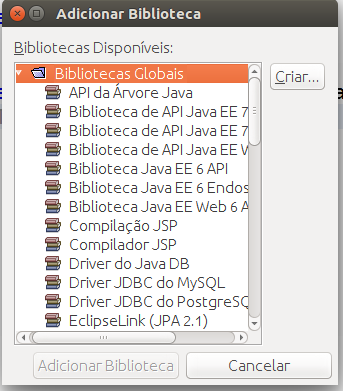
\includegraphics[height=0.5\paperheight]{fig/aula10/aula8_1.png}\\
% 	\tiny{\textbf{Fonte: }\cite{deitel2017java}}
      \end{center}
    \end{column}
%------------------------------
    \begin{column}{0.4\textwidth}
        \begin{enumerate}
	  \item Crie um projeto NetBeans Java;
	   \item Na guia \textbf{Projetos} do NetBeans;
	  \item Clique com o botão direito em \textbf{Bibliotecas}.
	   \item Adicionar Bibliotecas;
	   \item Escolha a biblioteca JDBC do banco que deseja utilizar;
	\end{enumerate}
   \end{column}
  \end{columns}
\end{frame}}
%----------------------------------------------------------------------
 \mode<presentation>{\begin{frame}{Banco}
 Utilize o script ``books.sql'' disponível no site da disciplina (\href{https://costasilvati.github.io/POO/}{https://costasilvati.github.io/POO/}) em Materiais de apoio.\\
 Crie e alimente o banco de dados.
\end{frame}}

%------------------------------------------------------------------------
 \mode<presentation>{\begin{frame}{Conexão com o banco}
\begin{center}
   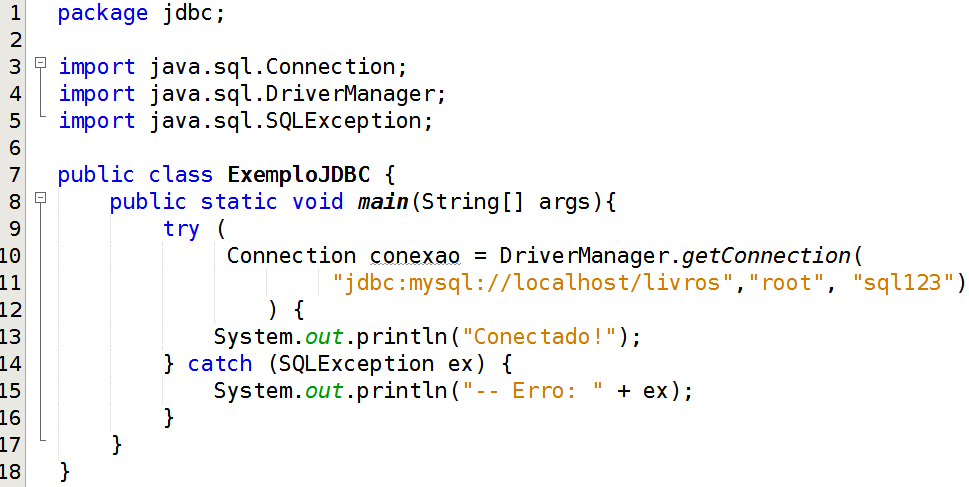
\includegraphics[height=0.57\paperheight]{fig/aula10/aula8_2.png} \\
%    \tiny{\textbf{Fonte: }\cite{deitel2017java}}
 \end{center}
  \small Se tudo correr bem, você verá o texto ``Conectado!''.
\end{frame}}

%------------------------------------------------------------------------
 \mode<presentation>{\begin{frame}{Fabrica de Conexões}
\begin{center}
   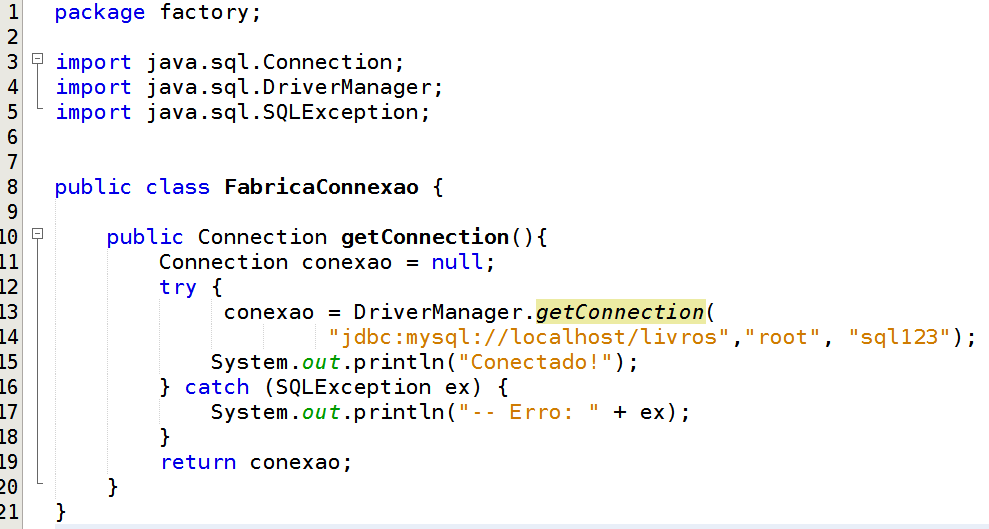
\includegraphics[height=0.57\paperheight]{fig/aula10/aula8_3.png} \\
%    \tiny{\textbf{Fonte: }\cite{deitel2017java}}
 \end{center}
  Precisa de uma conexão? Utilize:\\
 Connection con = new ConnectionFactory().getConnection();
\end{frame}}
%----------------------------------------------------------------
 \mode<presentation>{\begin{frame}{Realizando Consultas no banco}
  \begin{enumerate}
   \item Para realizar uma consulta é necessário criar um objeto do tipo 
Statement (que se faz as requisições SQL);
     \item Os resultados ficam em um objeto ResultSet;
     \item As informações sobre um objeto ResultSet são obtidas através 
do objeto ResultSetMetaData.
  \end{enumerate}
   Código disponível do site após a aula.
\end{frame}}

%----------------------------------------------------------------------
\section{Atividades}
 \mode<presentation>{\begin{frame}{Atividade}
 % Correção em: https://www.w3resource.com/java-exercises/collection/index.php#arraylist
 \tiny
 \textcolor{red}{\textbf{ATENÇÃO!} Atividades de 1 a 10 valem 500 pontos de Parcial. As atividades de 11 a 15, não são obrigatórias e valem 200 pontos extras.}\\
 Escreva um programa Java que contenha um menu, onde permita o usuário executar e ver os resultados das seguintes ações:
  \begin{enumerate}
  \item  Criar uma nova ArrayList, adicione algumas cores (string) e imprima a coleção. 
  \item Iterar através de todos os elementos de um ArrayList. 
  \item Inserir um elemento na ArrayList na primeira posição. 
  \item Recuperar um elemento (em um índice especificado) de uma determinada ArrayList.
  \item Atualizar um elemento específico do array por um elemento recebido pelo usuário.
  \item Remover o terceiro elemento de uma ArrayList e Procurar um elemento em uma ArrayList.
  \item Ordenar uma determinada ArrayList e Copiar uma ArrayList em outra. 
  \item Embaralhar elementos em uma ArrayList. 
  \item Inverter elementos em uma ArrayList e Extrair uma parte de uma ArrayList. 
  \item Comparar duas listas de array. 
  \item Troca de dois elementos selecionado pelo usuário em uma ArrayList e Juntar duas ArrayList. 
  \item Clonar uma ArrayList para outra ArrayList. 
  \item Esvaziar uma ArrayList e Testar se uma ArrayList está vazia ou não. 
  \item Alterar a capacidade de uma lista com o tamanho da lista atual ou Aumentar o tamanho de uma ArrayList. 
  \item Substituir o segundo elemento de uma ArrayList com o elemento especificado e Imprimir todos os elementos de uma ArrayList usando a posição dos elementos.
  \end{enumerate}

\end{frame}}
%******-----------------------------------------------------------------------
\section{Leitura recomendada}
 \mode<presentation>{
\begin{frame}{Leitura complementar}
 Para mais informações sobre JAVA, leia:\\
 \begin{columns}
   \begin{column}{0.4\textwidth}
     Java: Como programar\\
     \textbf{Capítulo 24}:\\ 
      \cite{deitel2010java}
   \end{column}
   \begin{column}{0.3\textwidth}
    \begin{center}
  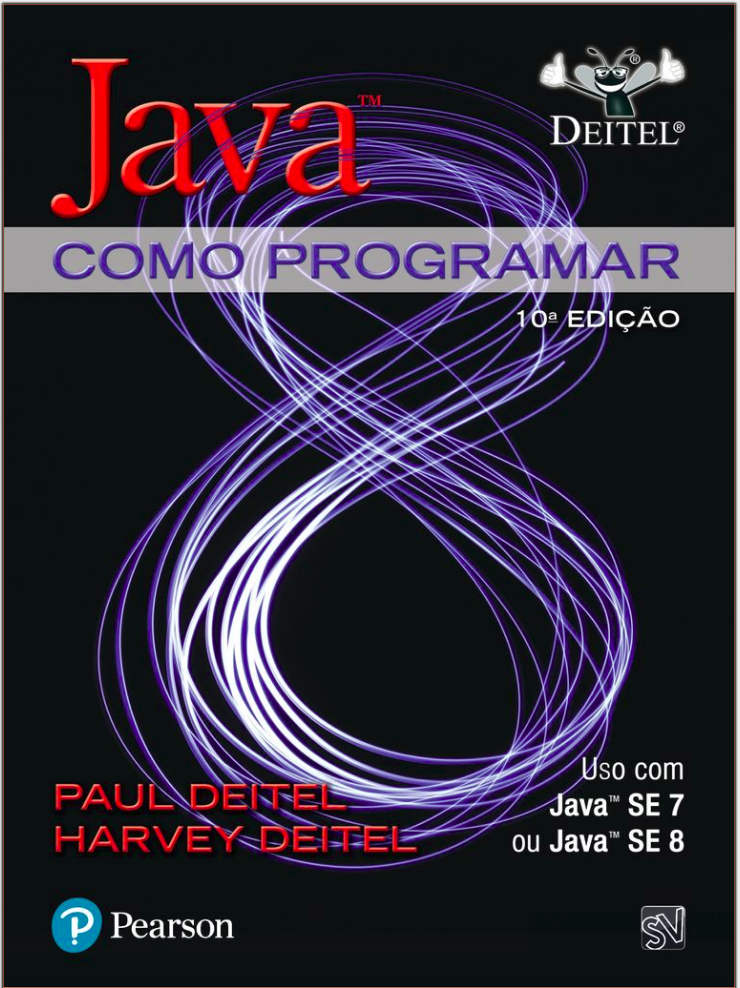
\includegraphics[height=0.5\paperheight]{fig/aula1/deitel2017java.png} \\
 \end{center}
   \end{column}
 \end{columns}
\end{frame}
}

%----------------------------------------------------------------------------------------------------------------------
 
 \mode<presentation>{\begin{frame}{Referências}%[allowframebreaks]
 \small
 \begin{center}
 	\bibliographystyle{apalike}
	 \bibliography{ref_aula_progI}
 \end{center}
 \end{frame}}


%%%%%%%%%%%%%%%%%% END MATTER %%%%%%%%%%%%%%%%%%
\end{document}